%% AAMAS 2027 main-track submission (GTEP), built on the official AAMAS-2027 template
%% (aamas.cls, AAMAS_2027_sample.tex). Figures in figures/ are exported from the interactive
%% explainer (light theme, vector PDF). Earlier versions: archive_acmart/, archive_storyled/.
%% acmthm=false is a documented class option: it keeps one counter per theorem kind, which the
%% main paper and the supplement cross-reference.

%%%% For anonymized submission, use this
\documentclass[sigconf,anonymous,acmthm=false]{aamas}

%%%% For camera-ready, use this (and paste the block from authors_camera_ready.tex)
%\documentclass[sigconf,acmthm=false]{aamas}

\usepackage{balance} % for balancing columns on the final page

%%%%%%%%%%%%%%%%%%%%%%%%%%%%%%%%%%%%%%%%%%%%%%%%%%%%%%%%%%%%%%%%%%%%%%%%

%%% AAMAS-2027 copyright block (do not change!)

\makeatletter
\gdef\@copyrightpermission{
  \begin{minipage}{0.2\columnwidth}
   \href{https://creativecommons.org/licenses/by/4.0/}{
\includegraphics[width=0.90\textwidth]{by}}
  \end{minipage}\hfill
  \begin{minipage}{0.8\columnwidth}
   \href{https://creativecommons.org/licenses/by/4.0/}{This work is licensed under a Creative Commons Attribution International 4.0 License.}
  \end{minipage}
  \vspace{5pt}
}
\makeatother

\setcopyright{ifaamas}
\acmConference[AAMAS 2027]{Proc.\@ of the 26th International Conference
on Autonomous Agents and Multiagent Systems (AAMAS 2027)}{3--7 May 2027}{Hanoi, Vietnam}{M.~Baldoni, F.~Fang, W.~Yeoh, N.~Yorke-Smith (eds.)}
\copyrightyear{2027}
\acmYear{2027}
\acmDOI{}
%\acmPrice{}
\acmISBN{}

%%%%%%%%%%%%%%%%%%%%%%%%%%%%%%%%%%%%%%%%%%%%%%%%%%%%%%%%%%%%%%%%%%%%%%%%

%%% OpenReview submission number: printed on the first page in anonymous mode.
% Set the actual OpenReview submission ID before submission.

\submissionType{Research Paper Track}

\usepackage{booktabs}
\usepackage{tabularx}
\usepackage{float}
\usepackage{graphicx}
\usepackage{subcaption}
\usepackage[capitalise,nameinlink]{cleveref}
\emergencystretch=1.5em
\renewcommand{\thefigure}{S\arabic{figure}}
\renewcommand{\thetable}{S\arabic{table}}

\theoremstyle{acmplain}
\newtheorem{slemma}{Lemma}
\renewcommand{\theslemma}{S\arabic{slemma}}
\newtheorem{sprop}{Proposition}
\renewcommand{\thesprop}{S\arabic{sprop}}
\newtheorem{stheorem}{Theorem}
\renewcommand{\thestheorem}{S\arabic{stheorem}}
\theoremstyle{acmdefinition}
\newtheorem{sremark}{Remark}
\renewcommand{\thesremark}{S\arabic{sremark}}

\newcommand{\E}{\mathbb{E}}
\newcommand{\TV}{\mathrm{TV}}
\newcommand{\dH}{d_{\mathrm{H}}}
\newcommand{\Kflat}{K_{\mathrm{flat}}}
\newcommand{\dmin}{d_{\min}}
\newcommand{\cube}{\{0,1\}}

\begin{document}
\title[How Much Memory Does Accountability Cost? (Supplement)]{Supplementary Material}
\subtitle{How Much Memory Does Accountability Cost? Incentives and Reconstruction from Bounded Multi-Agent Records}

\maketitle

Theorem, lemma and figure numbers without an ``S'' refer to the main paper, where all proofs appear in full; this supplement adds Theorem S1 on general priors, with its proof. Agents
\textsf{Alpha}, \textsf{Beta} and \textsf{Gamma} are agents 1, 2 and 3; profiles are written
in that order. Every figure is exported from the interactive explainer that accompanies the
paper, where each can be manipulated.

\appendix
\section{Proofs and Checks}

\subsection{Theorem 6: computational check}
The proof of Theorem 6 is in the main paper. \Cref{tab:orbit} compares the closed form with an
LP over $q$ for every reconstruction orbit, on a grid of $\mu$ spanning $[0,1/n]$. In every case the optimiser landed exactly on
$q^*(s)=\mu|s|+(1-n\mu)\mathbf1\{|s|>n/2\}$.

\begin{table}[h]
\caption{Theorem 6 against the exhaustive-orbit LP (Python 3.10.11, NumPy 2.2.6, SciPy 1.15.3).}
\label{tab:orbit}
\footnotesize
\begin{tabular}{@{}rrlr@{}}
\toprule
$n$ & $M_n$ & $\mu$ range & max deviation\\
\midrule
3 & 0.750000 & $[0,1/3]$ & 0\\
5 & 1.562500 & $[0,1/5]$ & 0\\
7 & 2.406250 & $[0,1/7]$ & $4.4\times10^{-16}$\\
9 & 3.269531 & $[0,1/9]$ & $3.1\times10^{-15}$\\
\bottomrule
\end{tabular}
\end{table}

\subsection{The threshold for every full-support prior}
Condition (M) never mentions the prior; only $D$ and $D_0$ do. Throughout, $N(s)$ is the set of
centres nearest to $s\notin C$, $N(c)=\{c\}$ for $c\in C$, and $\nu(s)=|N(s)|$. The record
spreads each profile uniformly over $N(s)$ and pays agent $i$ the $i$-th bit of the label's
centre.

\begin{stheorem}[The threshold for every full-support prior]\label{thm:prior}
For every full-support prior $\pi$, $\Kflat(\pi)$ is the least $K$ for which some
$\pi$-optimal $K$-median code has $\nu(s)\ge2$ for every $s\notin C$, and the record spreading
each profile uniformly over $N(s)$ attains it.
\end{stheorem}

\begin{slemma}[Margin of the construction]\label{lem:gen-margin}
Under every full-support prior $\pi$ and $\pi$-optimal code $C$, the record attains
$D=D_0(K)$ and its all-profile margin is $1-\max\nu(s')/\nu(s)$, where the maximum runs over
edges $\{s,s'\}$ with $d(s',C)=d(s,C)-1$; the margin is 1 if there are no such edges.
\end{slemma}
\begin{proof}[Proof sketch]
For an edge $s_1=s_0+e_i$, fixing a centre $c$ shows $d(s_0,c)$ and $d(s_1,c)$ differ by
one, according to $c_i$. Hence if the two profiles are equally far from $C$ their nearest
sets are disjoint, with $c_i=1$ on $N(s_1)$ and $c_i=0$ on $N(s_0)$, and the payment
separates them fully; if $s_1$ is closer, $N(s_1)\subseteq N(s_0)$ and the payment's
expectation moves from $\nu(s_1)/\nu(s_0)$ to 1; the reverse case is symmetric. The payment
puts $p_i=1$ exactly where $q[s_1,\cdot]$ exceeds $q[s_0,\cdot]$, so each edge attains its
total variation and Theorem 1's minimum is attained at a single edge.
\end{proof}

\begin{slemma}[Strict descent]\label{lem:strict-descent}
If $\nu(s)\ge2$ for every $s\notin C$, then $\nu(s')<\nu(s)$ on every edge with
$d(s',C)=d(s,C)-1$.
\end{slemma}
\begin{proof}
If $s'\in C$ then $\nu(s')=1<2$. Otherwise $r=d(s,C)\ge2$; translate so $s=0^n$ and
$s'=e_1$, so no centre has weight below $r$. $N(0^n)$ is the set of weight-$r$ centres and
$N(e_1)$ those among them with first bit 1, so equality would force every weight-$r$ centre
to carry that bit. Take one such centre $c$ and $y=c\oplus e_1$, of weight $r-1\ge1$, so
$y\notin C$ and $d(y,C)=1$. A centre adjacent to $y$ has weight $r$, hence carries the first
bit, which $y$ lacks, so it is $c$ itself: $\nu(y)=1$, a contradiction.
\end{proof}

\begin{proof}[Proof of Theorem S1]
Necessity: under full support $D_0$ is strictly decreasing for $K<2^n$, and the argument of
Lemma 1 applies at whatever radius the unique nearest centre lies. Sufficiency: by
\cref{lem:strict-descent}, $\nu(s')<\nu(s)$ on every edge on which $s'$ is one step closer to
$C$, so the margin $1-\max\nu(s')/\nu(s)$ of \cref{lem:gen-margin} is positive.
\end{proof}

Tilting can move the threshold either way (\cref{tab:prior}). When each agent works
independently with probability $0.7$ and $n=3$, the unique optimal 4-code is
$\{011,101,110,111\}$. It leaves $000$ at distance 2, yet the record is flat with $D=D_0(4)=0.2430$ and $\mu=1/3$ (main paper, Figure 4(c)). What the
prior decides is the structure of ties among optimal codes, not a direction: at $n=3$, $K=4$
the uniform prior has 62 optimal codes and the $0.7$ prior a single one. Both lemmas and the
theorem were checked by brute force on all 46,592 optimal codes at $n=3,4$ under uniform,
product and random priors, with no exceptions.

\begin{table}[h]
\caption{Least flat $K$ under the uniform and two tilted product priors, by Theorem S1,
confirmed by exhaustive search over prior-optimal codes.}
\label{tab:prior}
\footnotesize
\begin{tabular}{@{}lrrr@{}}
\toprule
 & uniform & $\Pr(S_i{=}1)=0.6$ & $\Pr(S_i{=}1)=0.7$\\
\midrule
$n=3$ & 4 & 6 & 4\\
$n=4$ & 7 & 13 & 5\\
\bottomrule
\end{tabular}
\end{table}

\subsection{Payments and memory}
Propositions 5 and 6 and their proofs are in the main paper; \cref{fig:sup-money} shows both.

\begin{figure}[h]
\centering
\begin{subfigure}[b]{\columnwidth}\centering
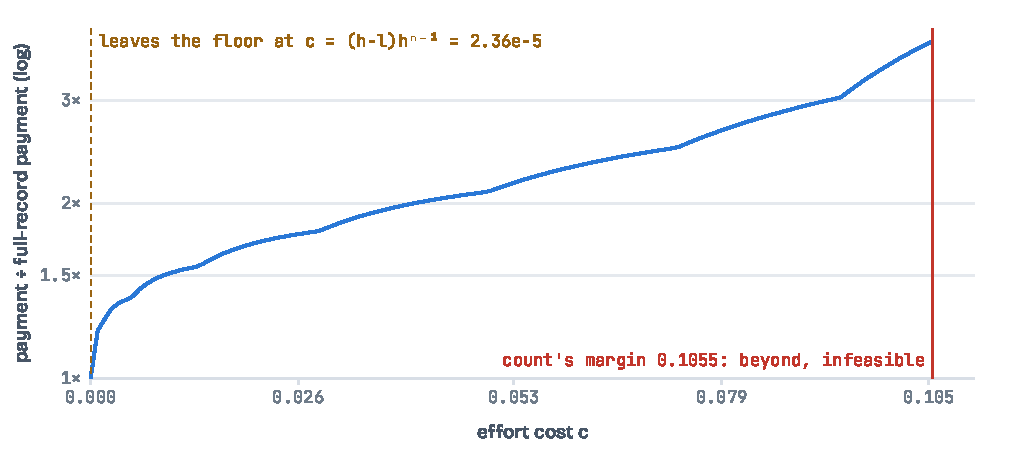
\includegraphics[width=\linewidth,page=1]{figures/cost.pdf}
\caption{Cost of a count record relative to the full record, $n=100$.}\end{subfigure}
\begin{subfigure}[b]{0.8\columnwidth}\centering
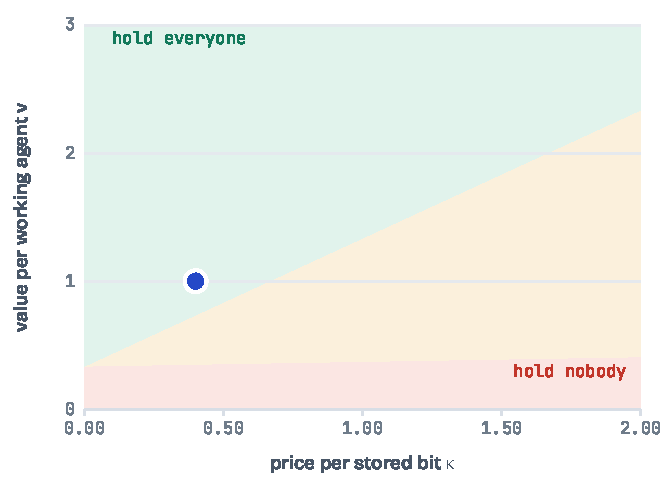
\includegraphics[width=\linewidth,page=1]{figures/designer.pdf}
\caption{The designer's regions at $c=0.3$.}\end{subfigure}
\caption{The price of accountability in payments and memory ($h=0.9$, $l=0.1$). (a) The
count leaves the cost floor once $c>(h-l)h^{n-1}$ and becomes infeasible beyond its margin
$0.1055$. (b) Hold nobody to account below the lower line, everyone with one bit each above
the upper line.}
\Description{Two charts. Top: payment of a success-count record divided by the full-record payment, on a logarithmic axis, against effort cost for 100 agents; it rises from 1 once cost exceeds a tiny threshold and the count becomes infeasible beyond its margin of 0.1055. Bottom: regions of a plane with price per stored bit on the horizontal axis and value per working agent on the vertical axis, separating hold nobody accountable, an intermediate region, and hold everyone accountable.}
\label{fig:sup-money}
\end{figure}

\section{Certificates and the Open Case}

\begin{table}[h]
\caption{Certificate chain. Shell: excluded by the shell bound (main paper, Lemma 3) without search. Infeasible:
2-domination integer program proved infeasible (not a time-out). Code: explicit 2-dominating
set, checked without a solver.}
\label{tab:cert}
\footnotesize
\begin{tabular}{@{}rllll@{}}
\toprule
$n$ & excluded & proved infeasible & attained & $\Kflat(n)$\\
\midrule
3 & $K\le3$ (shell) & -- & $K=4$ (code) & 4\\
5 & $K\le9$ (shell) & $K=9$ (redundant) & $K=10$ (code) & 10\\
7 & $K\le28$ (shell) & $K=29,30,31$ & $K=32$ (code) & 32\\
9 & $K\le93$ (shell) & $K=94,95,96$ & $K=128$ (code) & $[97,128]$\\
\bottomrule
\end{tabular}
\end{table}


\begin{figure*}[h]
\centering
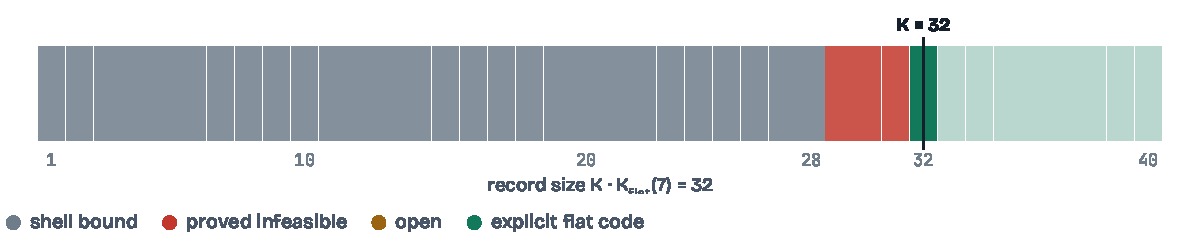
\includegraphics[width=0.8\textwidth,page=1]{figures/cert_chain.pdf}
\caption{Certificate chain at $n=7$. Grey: excluded by the shell bound with no search. Red:
2-domination integer program proved infeasible (not a time-out). Green: explicit
2-dominating set, checked without a solver. $\Kflat(7)=32$.}
\Description{A horizontal strip of cells for record sizes 1 to 40 at seven agents: grey cells up to 28 excluded by counting, red cells 29 to 31 proved infeasible, a highlighted green cell at 32 where an explicit flat code exists, and pale green cells above.}
\label{fig:cert}
\end{figure*}

\paragraph{Explicit codes.} At $n=5$ the explicit code gives $D=D_0=0.6875$, margin $0.5$,
$\dmin=2$. At $n=7$ it gives $D=D_0=0.75$, margin $0.5$, $\dmin=2$; this value has two
independent routes, the infeasibility chain and an algebraic parity-check construction. At
$n=9$ the explicit code gives $D=D_0=0.75$, margin $0.667$, $\dmin=3$.

\paragraph{Why $\Kflat(9)$ is open.} $\Kflat(9)\in[97,128]$. Feasibility integer programs at
$K=98,100,\dots,124$ (512 binaries) did not terminate within 40 minutes each; shrink-only
local search cannot move, because the algebraic code has no internal edges; and
destroy-and-repair search over 70,685 trials never improved on 128.

\paragraph{Bounds.} $2^{n+1}/(n+2)\le\gamma_2(Q_n)\le2^{\,n-\lfloor\log_2(n/2+1)\rfloor}$
(\cref{fig:gamma}). The lower bound is Fink and Jacobson's, attained at $n=3,5$; the upper
bound comes from a parity-check matrix with no zero column in which every nonzero syndrome
is used at least twice. The only claims that require a solver are the infeasibility of 2-domination at
$(n,K)=(5,9)$; $(7,29)$, $(7,30)$, $(7,31)$; and $(9,94)$, $(9,95)$, $(9,96)$.

\begin{figure}[h]
\centering
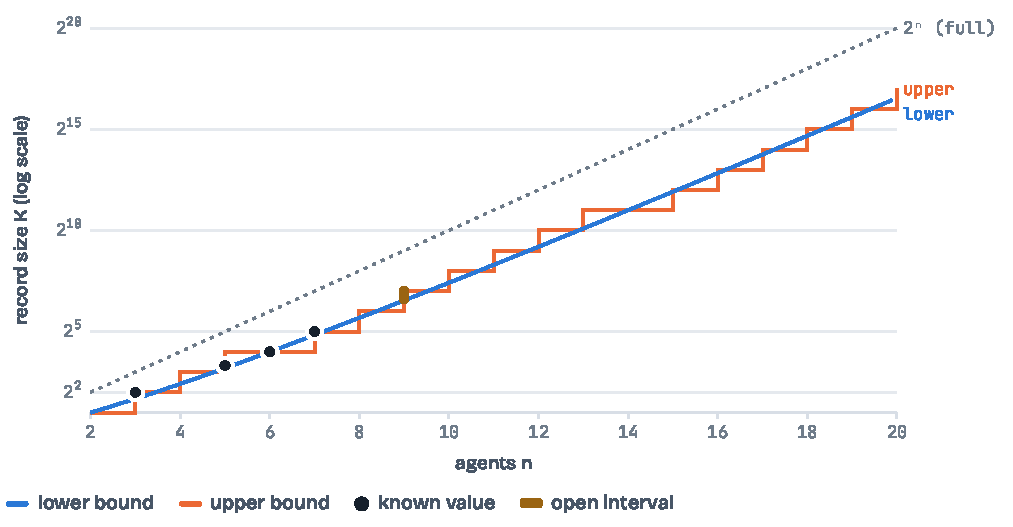
\includegraphics[width=\columnwidth,page=1]{figures/gamma.pdf}
\caption{Bounds on $\gamma_2(Q_n)$ (log scale). Dots are certified values; the bar at $n=9$
is the open interval.}
\Description{Logarithmic chart of the 2-domination number of the hypercube against the number of agents from 2 to 20, showing a lower-bound curve, a staircase upper bound, the full record size, known values as dots at 3, 5, 6 and 7 agents, and an open interval at 9 agents.}
\label{fig:gamma}
\end{figure}

\begin{table}[h]
\caption{Free compression under the uniform prior. $C(n)=2^n/\Kflat(n)$. At $n=20,50$ the
upper ends assume no flat record exists below $\gamma(Q_n)$.}
\label{tab:ratio}
\footnotesize
\begin{tabular}{@{}lrrrrrr@{}}
\toprule
$n$ & 3 & 5 & 7 & 9 & 20 & 50\\
\midrule
$C(n)$ & 2.00 & 3.20 & 4.00 & 4.00--5.28 & 8--11 & 16--26\\
free bits & 1.00 & 1.68 & 2.00 & 2.00--2.40 & 3.00--3.46 & 4.00--4.70\\
as \% of $n$ & 33.3 & 33.6 & 28.6 & 22--27 & 15.0--17.3 & 8.0--9.4\\
\bottomrule
\end{tabular}
\end{table}

\section{Additional Figures and Tables}
\begin{figure*}[t]
\centering
\begin{subfigure}[b]{0.3\textwidth}\centering
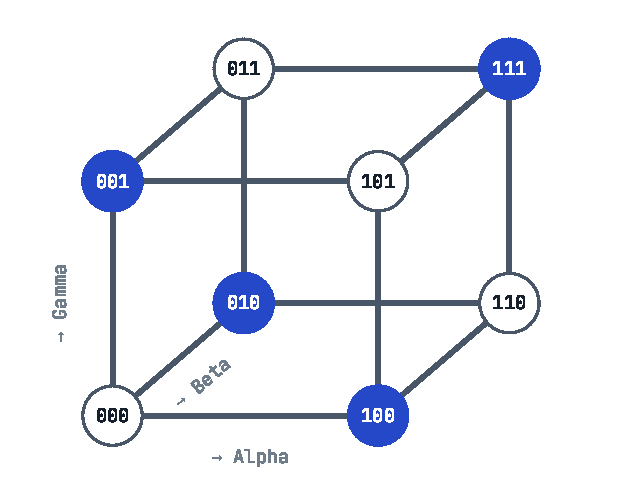
\includegraphics[width=\linewidth,page=1]{figures/g_cube_flat.pdf}
\caption{Flat: $D=0.5$, $\mu=2/3$.}\end{subfigure}\hfill
\begin{subfigure}[b]{0.3\textwidth}\centering
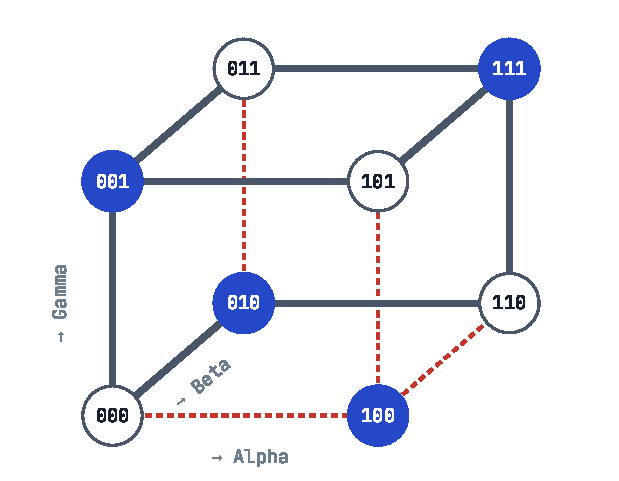
\includegraphics[width=\linewidth,page=1]{figures/g_cube_near.pdf}
\caption{Nearest centre: $D=0.5$, $\mu=0$.}\end{subfigure}\hfill
\begin{subfigure}[b]{0.3\textwidth}\centering
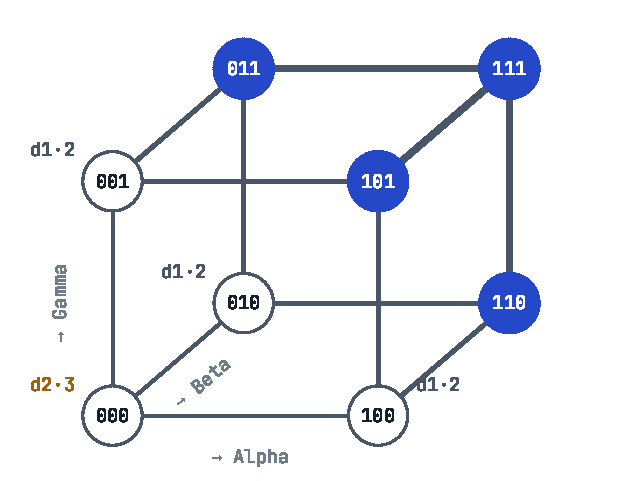
\includegraphics[width=\linewidth,page=1]{figures/g_cube_prior.pdf}
\caption{Bernoulli$(0.7)$ prior: flat, $\mu=1/3$.}\end{subfigure}
\caption{Records on the 3-cube; filled corners are centres and edge width is the total
variation across the edge. (a) The odd-weight class is 2-dominating, so spreading each other
corner over its three centre-neighbours is flat: $\Kflat(3)=\gamma_2(Q_3)=4$. (b) The same
centres with each corner sent to one nearest centre: same error, three dead edges (red), margin
0. (c) Under i.i.d.\ Bernoulli$(0.7)$ effort the unique optimal 4-code leaves $000$ at distance
2 with three nearest centres (label d2$\cdot$3); it is not 2-dominating, yet flat (Theorem S1).}
\Description{Three drawings of the 3-dimensional cube of effort profiles. Left: four filled centres forming the odd-weight class, all edges solid. Middle: the same centres with each other profile sent to one nearest centre; three edges are red and dashed, meaning one agent changing its effort leaves the record unchanged. Right: a different set of four centres for a tilted prior; profile 000 is at distance two from three centres, yet every edge is solid.}
\label{fig:cubes}
\end{figure*}

\begin{figure}[h]
\centering
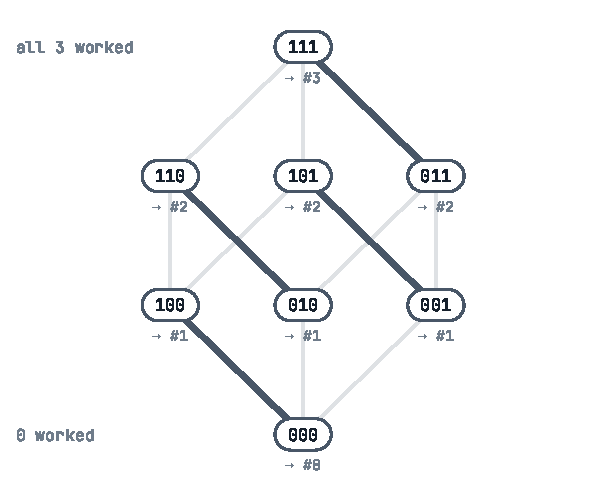
\includegraphics[width=0.85\columnwidth,page=1]{figures/lab_count.pdf}
\caption{The success count at $n=3$ on the effort lattice. Every edge in \textsf{Alpha}'s
direction moves the record, yet Theorem 1's adversary mixes teammate profiles so that the
teammate count is uniform, giving margin exactly $1/3$.}
\Description{Layered diagram of the eight effort profiles of three agents arranged by number of workers, with edges between profiles differing in one agent; every edge in the direction of the first agent changes the count label.}
\label{fig:lab}
\end{figure}

\begin{figure}[h]
\centering
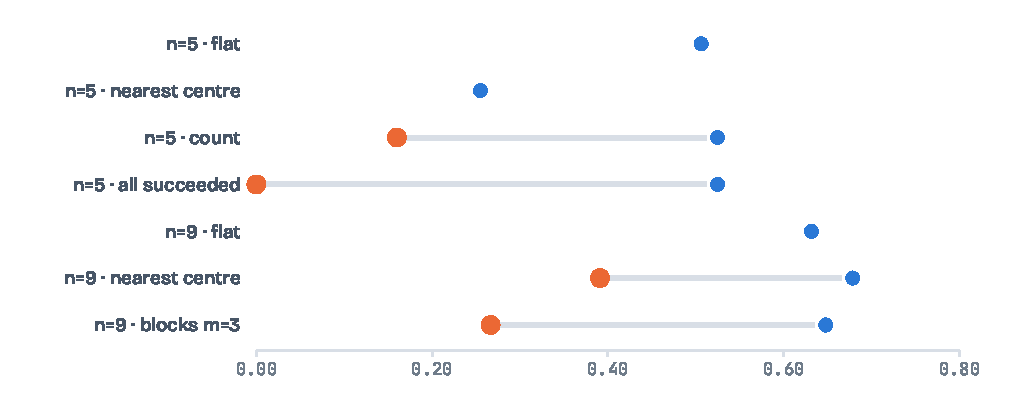
\includegraphics[width=\columnwidth,page=1]{figures/uniq.pdf}
\caption{Nash margin (blue) against dominant-strategy margin (orange) under noise, $h=0.9$, $l=0.1$.
Between the two, all-work is an equilibrium but other equilibria are not ruled out.}
\Description{Dumbbell chart for seven records comparing the Nash margin and the dominant-strategy margin under noise; for the flat records the two coincide, while the count and all-succeeded records have much smaller dominant-strategy margins.}
\label{fig:uniq}
\end{figure}

\begin{table}[h]
\caption{Exact Nash and dominant-strategy margins under noisy outcomes, $h=0.9$, $l=0.1$.}
\label{tab:noisy-exact}
\footnotesize
\begin{tabular}{@{}llrrr@{}}
\toprule
$n$ & record & $K$ & Nash & dominant-strategy\\
\midrule
5 & flat & 10 & 0.5063 & 0.5063\\
5 & nearest centre & 10 & 0.2550 & 0.2550\\
5 & count & 6 & 0.5249 & 0.1600\\
5 & all succeeded & 2 & 0.5249 & 0.0001\\
9 & flat & 128 & 0.6317 & 0.6317\\
9 & nearest centre & 128 & 0.6786 & 0.3911\\
9 & block counts, $m=3$ & 64 & 0.6480 & 0.2667\\
\bottomrule
\end{tabular}
\end{table}

\begin{table}[h]
\caption{Records of an episode trace, $n=5$, exact.}
\label{tab:episode}
\footnotesize
\begin{tabular}{@{}lrrrr@{}}
\toprule
record & $K$ & bits & $D$ & $\mu$\\
\midrule
full trace & 243 & 7.9 & 1.2500 & 0.5000\\
one bit per agent & 32 & 5.0 & 1.2500 & 0.5000\\
top-half agents only & 80 & 6.3 & 1.2923 & 0.2624\\
multiset of artifacts & 21 & 4.4 & 1.9718 & 0.1425\\
count of completions & 6 & 2.6 & 2.0194 & 0.1190\\
final output only & 2 & 1.0 & 2.1118 & 0.0243\\
\bottomrule
\end{tabular}
\end{table}

\begin{table}[h]
\caption{Attribution error on model-written reviews (192 episodes). The first and third rows
retain the same review texts; the third removes names and shuffles order.}
\label{tab:llm}
\footnotesize
\begin{tabular}{@{}lrr@{}}
\toprule
record & bytes & wrong agent labels (of 3)\\
\midrule
full trace & 2612 & 0.391\\
per-agent summary & 661 & 0.260\\
artifact multiset & 2582 & 1.333\\
global summary & 609 & 1.000\\
final output only & 507 & 1.193\\
\bottomrule
\end{tabular}
\end{table}

\paragraph{Model-written reviews, details.} The saved experiment uses
\texttt{codestral-2508} at temperature 0, with 24 episodes for each of the eight
assigned profiles (192 total), one fixed code diff, and three distinct fixed
review questions. Working is implemented by supplying the diff; shirking uses
a generic prompt without it. The historical system prompts describe incident
analysis although the user prompts supply a code review task. These are
experimentally assigned information conditions, not observed strategic effort
choices or incentive responses. The same model judges retained records.
The artifact-multiset transformation removes labels \emph{and shuffles order};
it does not isolate the causal effect of name removal. Questions and agent
positions are confounded, and heterogeneous content can reveal identity even
after names are removed.

The error is Hamming loss on three binary agent labels, not entropy or stored
bits. Taking the best of the $3!$ permutations of each judge answer reduces
the multiset error from 1.333 to 0.438, its count error. The paired mean gap
against the full trace is 0.943 wrong labels (episode-bootstrap 95\% interval
$[0.802,1.089]$); this interval describes resampling of the collected episodes,
not generalisation to other tasks, models, or role assignments.

The empirical channel maps the assigned profile to the \emph{judge's predicted
profile}; its alphabet has at most eight outcomes regardless of text length.
Margins and Bayes errors computed from this channel concern the judge's
compression, not the maximum incentives attainable from raw text. Finite-sample
margin errors can have either sign. At four episodes per profile, seven
identical empirical conditional-distribution pairs forced an estimated zero
full-trace margin; no such ties remained at 24 episodes. This is not a
one-sided statistical bound. The estimated multiset margin (0.207) exceeds
the full-trace margin (0.075), reversing the preregistered ordering. We retain
this negative result and make no causal claim that identity removal reduces
incentives in this experiment.

\paragraph{Verification scope.} The revision reruns the solver-free suite
\texttt{src/verify\_all.py} and the checks in \texttt{experiments/},
\texttt{threshold\_tightness.py} and
\texttt{repeated\_review.py}. All pass. These check finite instances,
numerical formulae, and supplied constructions; they do not replace the proofs
or independently reproduce every optimisation certificate and model API call.
The theorem on threshold tightness has an asymptotic constant at fixed noise
parameters and vanishing effort cost, with finite-size rounding as stated in
the main paper. The repeated-review result assumes a committed effort plan
without intermediate feedback and bounds final record size, not online
working memory. The general flatness equality in the main paper is restricted
to the dominating-code regime; Theorem S1 gives the unrestricted prior-specific
characterisation.

\section{Pre-registered Predictions}
Of 22 registered predictions, 8 were derivations whose failure would have meant a false
theorem or a bug; all 8 held. Of 14 conjectures, 11 were falsified (\cref{tab:prereg}). Each
was hashed before its harness was written.

\begin{table*}[h]
\caption{Pre-registered conjectures that were falsified (11 of 14).}
\label{tab:prereg}
\footnotesize
\begin{tabularx}{\textwidth}{@{}>{\raggedright\arraybackslash}p{70mm}>{\raggedright\arraybackslash}X@{}}
\toprule
prediction & outcome and reason\\
\midrule
The count has full margin (one deviation always moves it by one) & Margin exactly $1/n$: the minimax mixes teammate counts uniformly, and intermediate shifts cancel.\\
Margins fall monotonically with observation noise $\eta$ & The flat record rises $0.5000\to0.5196$ at $\eta=0.05$ before falling: noise spreads each flip over labels.\\
Noise cannot create margin where a deterministic record has none & $K$-median $0\to0.1973$ ($n=5$), threshold $0\to0.1440$ ($n=3$) at $\eta=0.1$.\\
Identity-removal ratio exceeds 3 in every matched comparison & Minimum 1.07, median 1.4--2.3; the direction held, the magnitude did not.\\
That ratio grows with $n$ & No consistent growth over $n=3,\dots,7$.\\
Top-half-agents record has margin exactly 0 & 0.2624: selection depends on behaviour, so shirking changes an agent's chance of being recorded.\\
Ship/no-ship bit has zero margin & 0.0900 ($n=3$), 0.0243 ($n=5$), decaying in $n$.\\
Margin ordering of records holds over all three model-written agents & Fails over three agents; holds over the two comparable ones. The third sub-task is far less auditable (accuracy 0.677).\\
Artifact multiset has a margin smaller than the full trace by at least a third & Reversed: 0.207 against 0.075; the full trace's margin is set by the hard-to-audit third agent.\\
Final output only has a margin near zero but not exactly zero & Exactly zero at 192 episodes.\\
Multiset error close to the full trace's while its margin is not & Error 1.333 against 0.391 wrong agent labels: the multiset matches the full trace on how many (0.438 against 0.391), not on which.\\
\bottomrule
\end{tabularx}
\end{table*}


\paragraph{Relation to prior work.} Monitoring and information structures are
endogenous in parts of the contracting and information-design literature.
Our restriction is specifically the finite alphabet of the retained public
record, combined with bounded payments and a reconstruction objective. The
main paper distinguishes the standard total-variation/minimax and information
inequality tools from the threshold construction, attribution bound, and
nearest-centre geometry studied here.

\end{document}
